\section{Versuchsaufbau/-durchführung}
Bei den Teilversuchen \emph{Zeitabhängigkeit der Schwingungsamplitude}
und \emph{Widerstandsbestimmung für den ap. Grenzfall} wird der selbe
Versuchsaufbau \ref{fig:aufbau_eins} verwendet. Lediglich der Widerstand ist bei dem
zweiten Teilversuch variabel einstellbar.
\begin{figure}
  \centering
  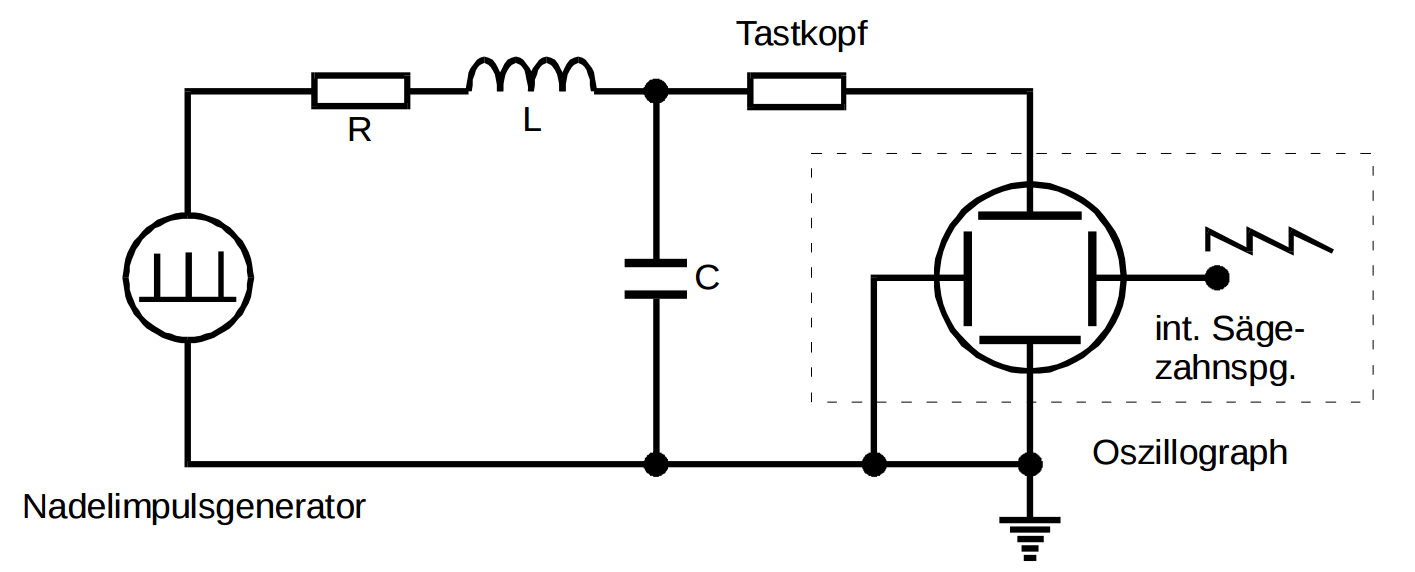
\includegraphics[width = 0.5\textwidth]{bilder/erster_versuchsaufbau.png}
  \caption{Versuchsaufbau für die Untersuchung der Schwingungsamplitude und des ap. Grenzfalles \cite{anleitung354}. }
  \label{fig:aufbau_eins}
\end{figure}
Die in der Abbildung zusehende Spule $L$ und der Kondensator $C$ werden verwendet, um
ein schwingfähiges System zu konstruieren. Eine Dämpfung der Schwingung
erfolgt mittels des Widerstandes $R$ (später variabel einstellbar).
Der Nadelpulsgenerator dient zur Anregung des Systems. Seine Frequenz wird so
eingestellt, dass eine Untersuchung des Schwingverhalten mit Hilfe des
Ozilloskops möglich ist. Die für den Versuch verbauten Bauteile besitzen folgende
Werte:
\begin{align}
  \label{eq:bauelemente_1}
  \begin{aligned}
    L=\SI{10.11}{\milli\henry}\\
    C=\SI{2.098}{\nano\farad}
  \end{aligned}
\end{align}
\subsection{Zeitabhängigkeit der Schwingungsamplitude}
Am Anfang wird das Entladeverhalten des Kondensators beim Schwingfall betrachtet.
Die Frequenz des Generators muss %Generators
so eingestellt werden, dass die Kondensatorspannung um den Faktor $3$ bis $8$
abnimmt, bevor ein wiederholter Peak das System erneut anregt.
Mit Hilfe der 'Cursor'-Funktion des Oszilloskops, wird dann %Mit Hilfe, beides ist möglich
die Höhe von allen oberen Schwingungsmaxima gemessen.
Der hier verwendete Widerstand hat einen Wert von $R=\SI{48.1}{\ohm}$.
\subsection{Widerstandsbestimmung für den ap. Grenzfall}
Bei diesem Teilversuch soll ein variabele Widerstand $R$ ($R\ua{max}=\SI{5}{\kilo\ohm}$) so eingestellt werden,
dass der aperiodische Grenzfall beobachtet werden kann.
Hierzu wird zunächst das Potentionmeter auf seinen Maximalwert justiert.
Der Widerstand wird nun kontinuierlich verringert, dabei wird das %verringert
Ozsilloskop beobachtet. Man dreht den Widerstand so weit runter, bis %so weit
ein Überschwinger ($\frac{\map{d}U\ua{C}}{\map{d}t}>0$) entdeckt wird.
Der Widerstand wird nun soweit erhöht, bis der Überschwinger gerade verschwindet.
An dieser Stelle befindet sich der aperiodische Grenzfall und somit $R\ua{ap}$. %befindet, aperiodische
\subsection{Frequenzabhängigkeit der Kondensatorspannung und Phase}
\begin{figure}
  \centering
  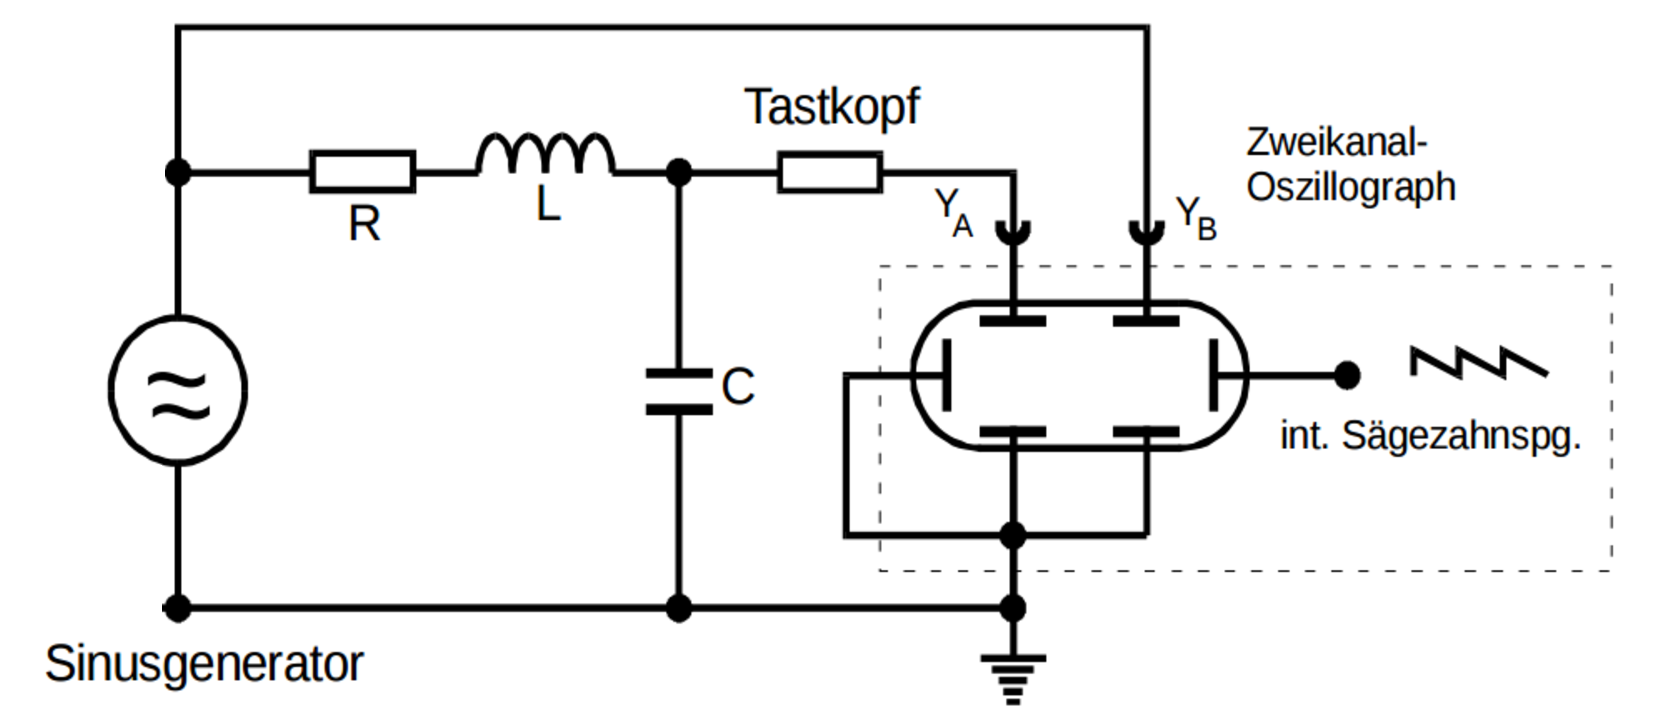
\includegraphics[width = 0.5\textwidth]{bilder/aufbau_zwei.pdf}
  \caption{Versuchsaufbau für die Untersuchung der Frequenzabhängigkeit der Kondensatorspannung und Phase \cite{anleitung354}. }
  \label{fig:aufbau_zwei}
\end{figure}
Der Versuch wird nach Abbildung \ref{fig:aufbau_zwei} aufgebaut.
Der Unterschied zu Abbildung \ref{fig:aufbau_eins} liegt zum einem
in der Veränderung des Widerstands auf $R=\SI{509.5}{\ohm}$ zum andern, wird
auf dem Oszilloskop zusätzlich die Generatorspannung angezeigt.
Die am Generator anliegende Frequenz wird im Intervall $f\in\left[25,45\right]\,\si{\kilo\hertz}$
varriiert und mit dem Oszilloskop gemessen. Bei der vom Generator erzeugten Spannung handelt es sich um
eine Sinusspanunng. Mit Hilfe der 'Measure'-Funktion des Ozsilloskops %Mit Hilfe, Oszilloskops
kann Generator- und Kondensatorspannung bei verschiedenen Frequenzen %verschiedenen
abgelesen werden. Zusätzlich wird mit ihr die Phasenlänge $b$ der Generatorspannung
gemessen. Abschließend bietet die 'Cursor'-Funktion eine Möglichkeit %ohne um
die zeitliche Differenz $a$ zwischen Generator- und Kondensatorspannung zu
bestimmen.
Mit den Größen $a$ und $b$ kann dann der Phasenunterschied zwischen
Generator- und Kondensatorspannung errechnet werden:
\begin{equation}
  \label{eq:phasen_unterschied}
  \varphi=\frac{2a}{b}\pi.
\end{equation}
%schau mal in die pdf, an vielen Stellen sind Zeilen eingerückt
